% Umbrella for the five geometric features (refactored 2026-11-06, user). Each feature is a
% \subsection in its own file, input in this order:
%   05a_curvature.tex           sec:method-curvature
%   05b_bifurcation_angle.tex   sec:method-angle
%   05c_daughter_ratio.tex      sec:method-ratio
%   05d_taper.tex               sec:method-taper
% 2026-11-06 (thesis-style pass): heading to sentence case; ostium gloss cut (defined in
%   sec:circulation); trailing "Taper also needs" sentence folded into the per-segment sentence;
%   "lumen radius" and "lumen mask" removed pending code, see the two \clarify notes.
% CHECK: thesis_final/ holds only turning_feature.py and split_check.py; taper, angle and ratios
%   have no final script yet.
% 2026-11-06 (user): opening rewritten. Many ways to quantify geometry, so features restricted to
%   those the literature points to; one-sentence recap of sec:method-selection, which it does not repeat.
% Shared rules live here: unit of measurement (written), missing values (TODO).
% Does not repeat: why the features are computed per segment (02b_segment_split.tex), how they enter
%   the model (03_prediction_model.tex), why these five were chosen (04_model_size.tex,
%   sec:method-selection).
\providecommand{\clarify}[1]{\textcolor{red}{\textbf{Clarification needed:} #1}}
\section{Geometric features}
\label{sec:method-features}

A large number of descriptors are used to try to capture the geometry of coronary arteries.
The features used in this thesis were drawn from the studies that have associated coronary geometry with low WSS or with plaque location (Chapter~\ref{ch:literature}, Section~\ref{sec:method-selection}).



Some were adapted from the measures used in these studies, such as curvature, which is computed here on 3D centerlines over a fixed chord rather than on 2D angiograms (Section~\ref{sec:method-curvature}).
The five resulting features are summarized in Table~\ref{tab:method-features} and illustrated in Figure~\ref{fig:method-features}.
They were read from the arteries of Section~\ref{sec:method-split}, in which every point carries a position in millimeters and an artery label.
To count distance along an artery from the same anatomical point in every participant, each artery was traversed from its ostium, taken as the uppermost end of the tree.
\clarify{In \texttt{split\_trunks.py} (\texttt{trunk\_path}) the LAD and LCx paths start at the left main bifurcation after the split, not at the ostium; only the RCA starts at the ostium. Which start do the features use?}
Curvature was computed from the centerline points of each of the nine segments and taper from the lumen cross-sections along them, while the bifurcation angle and the two diameter ratios were computed once per participant at the left main bifurcation.
\clarify{The split points carry no lumen radius in \texttt{split\_trunks.py}, and the tracer gives a lumen contour per step rather than a mask. No script in \texttt{CGPS\_data/thesis\_final/} yet computes taper, the angle or the ratios, so their inputs are unconfirmed.}

\begin{table}[htbp]
  \centering
  \caption{The five geometric features. All are read from the labeled centerline tree; taper also needs the lumen cross-sections along it.}
  \label{tab:method-features}
  \begin{tabular}{llll}
    \toprule
    Feature & Measured on & Input & Section \\
    \midrule
    Turning-angle curvature & each segment & centerline points & \ref{sec:method-curvature} \\
    Bifurcation angle & left main bifurcation & daughter directions & \ref{sec:method-angle} \\
    Diameter ratios LM to LAD and LM to LCx & left main bifurcation & parent and daughter radii & \ref{sec:method-ratio} \\
    Taper & each segment & lumen cross-sections & \ref{sec:method-taper} \\
    \bottomrule
  \end{tabular}
\end{table}

% Figure from features_overview_schematic.py (made-up left coronary tree, no patient data). Panels A,
% B and D run the thesis code (turning_feature.py, lm_bifurcation_angle, tortuosity/taper.py); panel C
% has no code behind it, see the \clarify notes in 05c_daughter_ratio.tex and below.
\begin{figure}[htbp]
  \centering
  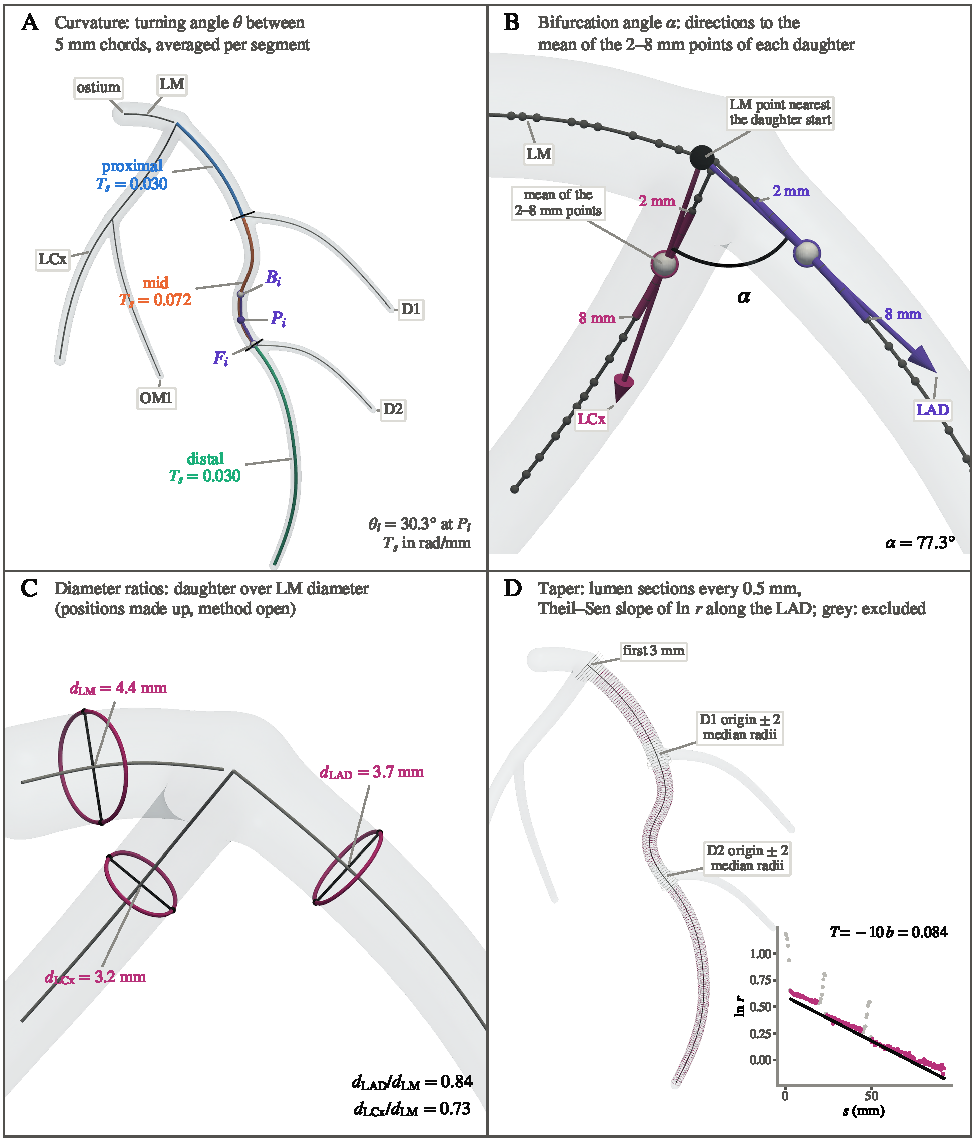
\includegraphics[width=\textwidth]{methodology/features_overview_schematic.pdf}
  \caption{The four geometric features on a made-up left coronary tree, drawn as a semi-transparent lumen with its centerline. (A) Curvature: the LAD is divided at the D1 and D2 origins (black rings) into a proximal, a mid and a distal segment, and at every centerline point $P_i$ the turning angle $\theta_i$ is measured between the 5\,mm chords to $B_i$ and $F_i$; $T_s$ is the arc-length mean of $\theta/\ell$ over each segment, in rad/mm (Section~\ref{sec:method-curvature}). (B) Bifurcation angle: $\alpha$ is the angle between the directions from the left main point nearest the start of each daughter to the mean of the daughter's centerline points 2 to 8\,mm along it (Section~\ref{sec:method-angle}). (C) Diameter ratios: the LAD and LCx diameters divided by the left main diameter, here at made-up positions (Section~\ref{sec:method-ratio}). (D) Taper: the lumen is cut every 0.5\,mm orthogonal to the centerline, sections in the first 3\,mm and within two median radii of a branch origin are excluded (grey), and $T = -10\,b$, where $b$ is the Theil--Sen slope of $\ln r$ against arc length $s$ (inset), is the fractional loss of radius per 10\,mm (Section~\ref{sec:method-taper}). All values are computed on the made-up tree.}
  \label{fig:method-features}
\end{figure}
\clarify{Figure~\ref{fig:method-features}C shows the diameters at made-up positions, since where and how the left main and daughter diameters are measured is not yet defined; panel D computes taper on the whole LAD, as \texttt{tortuosity/taper.py} does, not per segment (see Section~\ref{sec:method-taper}).}
